% Third Golden Rule of Bioinformatics Exercise
%
% The aim of this exercise is to demonstrate that a simple question 
% of biological relevance does not have the obvious answer. The point
% is to reinforce that even "simple" questions may require sufficient 
% thought and attention, in order to answer them properly. Also, that 
% "intuition" is not always sufficient for even "simple" questions.

\subsection{Golden Rule 3 Exercise}
\begin{frame}
  \frametitle{Exercise 3}
  \framesubtitle{Classification}
  \begin{itemize}
    \item Rule: If there is a vowel on one side of a card, there \textit{must} be an even number on the other side of that card.
    \item Is this rule true?
    \item Which cards, when turned over, can help determine if this rule is true? (How many are there?)
  \end{itemize}
  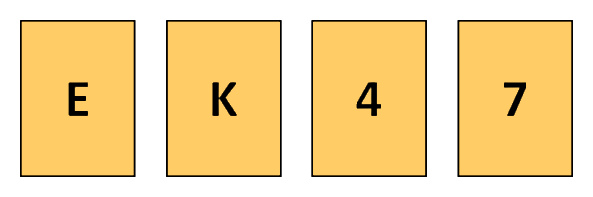
\includegraphics[width=0.8\textwidth]{images/wason}
\end{frame}

\subsection{Golden Rule 3 Exercise}
\begin{frame}
  \frametitle{Exercise 3}
  \framesubtitle{Classification}
  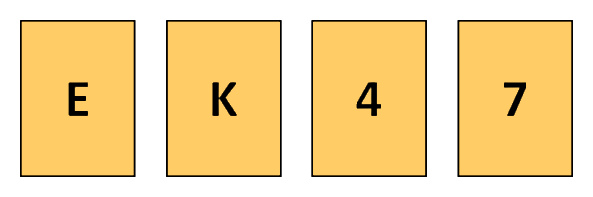
\includegraphics[width=0.8\textwidth]{images/wason}
\end{frame}

\begin{frame}
  \frametitle{Exercise 3}
  \framesubtitle{Classification}
  This is the Wason Selection Task
  \begin{itemize}
    \item<1-> If you chose \emph{E} and \emph{4}
    \begin{itemize}
      \item<2-> You are in the typical majority group
      \item<2-> You are not correct
      \item<2-> You have been a victim of confirmation bias (System 1 thinking)
    \end{itemize}
    \item<3-> If you chose \emph{E} and \emph{7}
    \begin{itemize}
      \item<4-> Congratulations!
      \item<4-> Your choice was capable of \textit{falsifying} the rule.
    \end{itemize}
  \end{itemize}
\end{frame}

\begin{frame}
  \frametitle{Exercise 3}
  \framesubtitle{Classification}
  Rule: If there is a vowel on one side of the card, there \textit{must} be an even number on the other side.    
  \begin{center}
  \begin{tabular}{c|c|c}
	  Card & Outcome & Rule \\
	  \hline
	  \hline
	    \multirow{2}{*}{E} & Even & Can be true even if rule false \\
	                                & Odd & \emph{violated} \\
	  \hline
	    \multirow{2}{*}{K} & Even & na \\
	                                & Odd & na \\	    
	  \hline
	    \multirow{2}{*}{4} & Vowel & Can be true even if rule false \\
	                                & Consonant & na \\
	  \hline
	    \multirow{2}{*}{7} & Vowel & \emph{violated} \\
	                                & Consonant & na \\	    
  \end{tabular}
  \end{center}
\end{frame}

\begin{frame}
  \frametitle{Exercise 3}
  \framesubtitle{Classification}
  \begin{itemize}
    \item This is equivalent to functional classification, e.g:
    \item Rule: If there is a CRN/RxLR/T3SS domain, the protein \textit{must} be an effector.
  \end{itemize}
  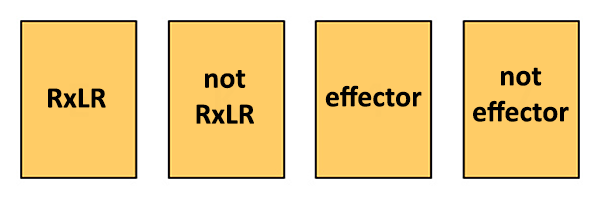
\includegraphics[width=\textwidth]{images/wason_rxlr}
\end{frame}
  
\begin{frame}
  \frametitle{Exercise 3}
  \framesubtitle{Classification}
  \begin{itemize}
    \item Confirmation Bias (Wason Selection Task)
    \begin{itemize}
      \item An uninformative experiment is performed
      \item \url{http://en.wikipedia.org/wiki/Wason_selection_task}
    \end{itemize}
    \item Affirming the Consequent (a related formal fallacy)
    \begin{enumerate}
     \item If $P$, then $Q$
     \item $Q$
     \item Therefore, $P$
    \end{enumerate}
    \begin{itemize}
      \item Experimental results are misinterpreted
      \item \url{http://en.wikipedia.org/wiki/Affirming_the_consequent}
    \end{itemize}
  \end{itemize}
\end{frame}
